\newgeometry{top=15truemm,bottom=15truemm,left=20truemm,right=20truemm}
\chapter{第\ref{chap:upper-bound}章の補足}

% \section{補題\ref{lem:variance-inequality}の証明}\label{sec:prf-lemma-variance-inequality}
% \begin{screen}
    % \begin{lemma}
    %     分散についての以下の不等式が成り立つ。
    %     \begin{align}
    %         \Var\Big[\sum_i X_i\Big] &\leq N\sum_i\Var[X_i],\\
    %         \Var[XY] &\leq 2\Var[X]\abs{Y^2}_{\max} + 2(\E[X])^2\Var[Y]\,.
    %     \end{align}
    % \end{lemma}
% \end{screen}

% \begin{proof}
%     We have
%     $$
%     \begin{aligned}
%     \operatorname{Var}[X+Y] & =\operatorname{Var}[X]+\operatorname{Var}[Y]+2 \operatorname{Cov}[X, Y] \\
%     & \leqslant \operatorname{Var}[X]+\operatorname{Var}[Y]+2 \sqrt{\operatorname{Var}[X] \operatorname{Var}[Y]} \\
%     & \leqslant \operatorname{Var}[X]+\operatorname{Var}[Y]+\sqrt{\operatorname{Var}[X] \operatorname{Var}[X]}+\sqrt{\operatorname{Var}[Y] \operatorname{Var}[Y]} \\
%     & =2 \operatorname{Var}[X]+2 \operatorname{Var}[Y]
%     \end{aligned}
%     $$
%     32
%     where in the first inequality we have used Cauchy-Schwarz, and the second inequality comes from the rearrangement inequality. Now consider
%     $$
%     \begin{aligned}
%     \operatorname{Var}[X Y] & =\operatorname{Var}[(X-\mathbb{E}[X]) Y+\mathbb{E}[X] Y] \\
%     & \leqslant 2 \operatorname{Var}[(X-\mathbb{E}[X]) Y]+2 \operatorname{Var}[\mathbb{E}[X] Y] \\
%     & \leqslant 2 \mathbb{E}\left[(X-\mathbb{E}[X])^2 Y^2\right]+2(\mathbb{E}[X])^2 \operatorname{Var}[Y] \\
%     & \leqslant 2 \mathbb{E}\left[(X-\mathbb{E}[X])^2\right]\left|Y^2\right|_{\text {max }}+2(\mathbb{E}[X])^2 \operatorname{Var}[Y] \\
%     & =2 \operatorname{Var}[X]\left|Y^2\right|_{\text {max }}+2(\mathbb{E}[X])^2 \operatorname{Var}[Y]
%     \end{aligned}
%     $$
%     where in the first inequality we have used Eq. (G5), in the second inequality we have used the definition of the variance, and in the third inequality we have simply taken the maximum value for $Y^2$.
% \end{proof}

\section{ローカルユニタリ $2$--デザイン: ALT の計算例}\label{sec:alt-calculation}
ここでは、ローカルユニタリ $2$--デザインの仮定の下での $\int_{U\in\bbU} dU D_{\HS} (\rho^{(h)} , \bbid/2^s)$ の計算について、量子ビット数が $6$、層数が $3$、$s = 1$ の場合の例を用いて説明する。
$D_{\HS} (\rho^{(h)} , \bbid/2^s) = \operatorname{Tr}[(\rho^{(h)})^2] - 1/2^s$ であるから、$\int_{U\in\bbU} dU \operatorname{Tr}[(\rho^{(h)})^2]$ を計算すれば良い。$\operatorname{Tr}[(\rho^{(h)})^2]$ をテンソルネットワークで表現すると、図~\ref{fig:tn-alt-int-1} の一番上のネットワークのようになる。これを、各ゲートブロックがユニタリ $2$--デザインを成すとして積分する。
以降の図では、$UU\dg = \bbid$ となって消える部分を灰色で表現している。図の最初の等号では、灰色の部分を消した。
2つ目の等号は、$U_1$ のみを、図~\ref{fig:haar-int-4}を用いて積分した。
\begin{figure}[H]
    \centering
    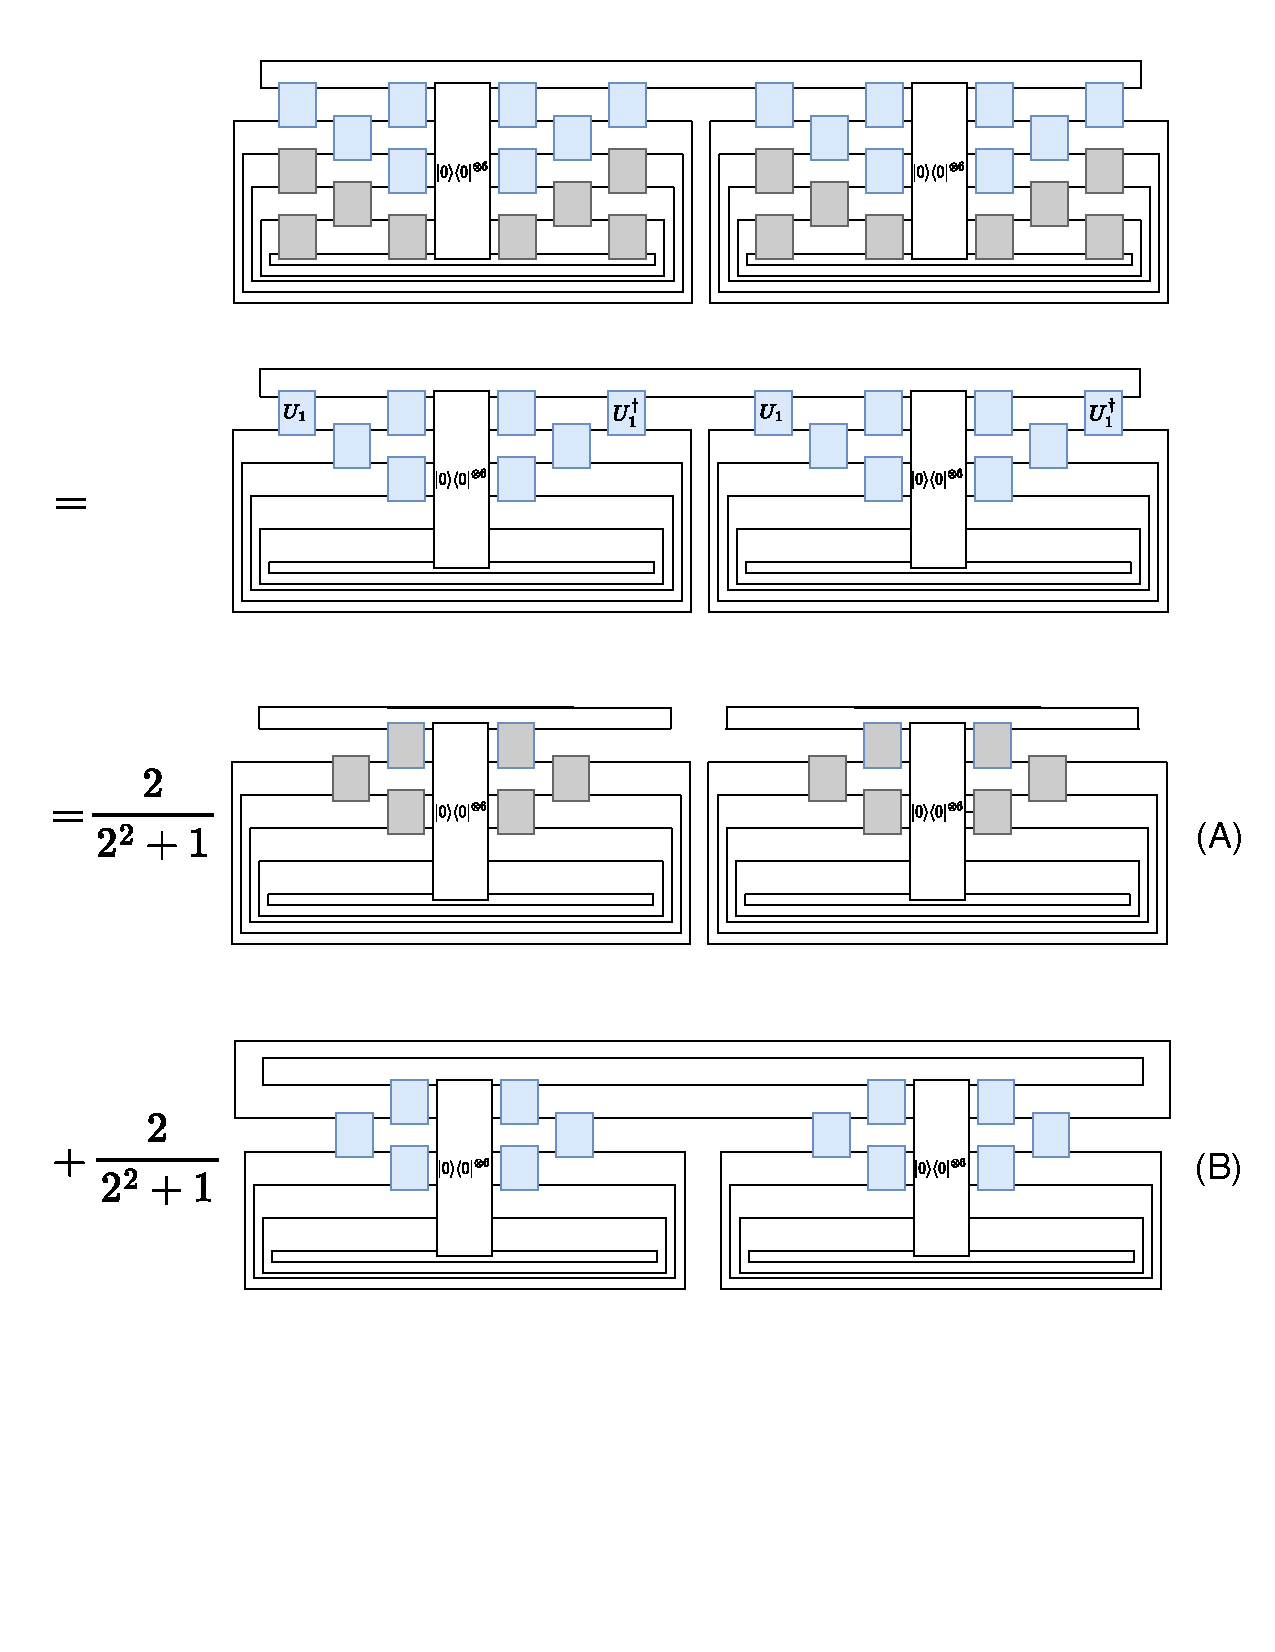
\includegraphics[width=15cm]{int-ALT-Page-1.drawio.pdf}
    \vspace{-20pt}
    \caption{量子ビット数が $6$、層数が $3$、$s = 1$ の ALT において、$U_1$ を図~\ref{fig:haar-int-4}を用いて積分}
    \label{fig:tn-alt-int-1}
\end{figure}

これにより出てきた2つの項(A)と(B)について:まず、項(A)は $(\operatorname{Tr}[U\dyad{0}\otn{6}U\dg])^2 = 1$ である。次に項(B)については、図~\ref{fig:tn-alt-int-2}の一番上のネットワークのゲートブロック $U_2$ を積分すると項(C), (D)に分解される。
\begin{figure}[H]
    \centering
    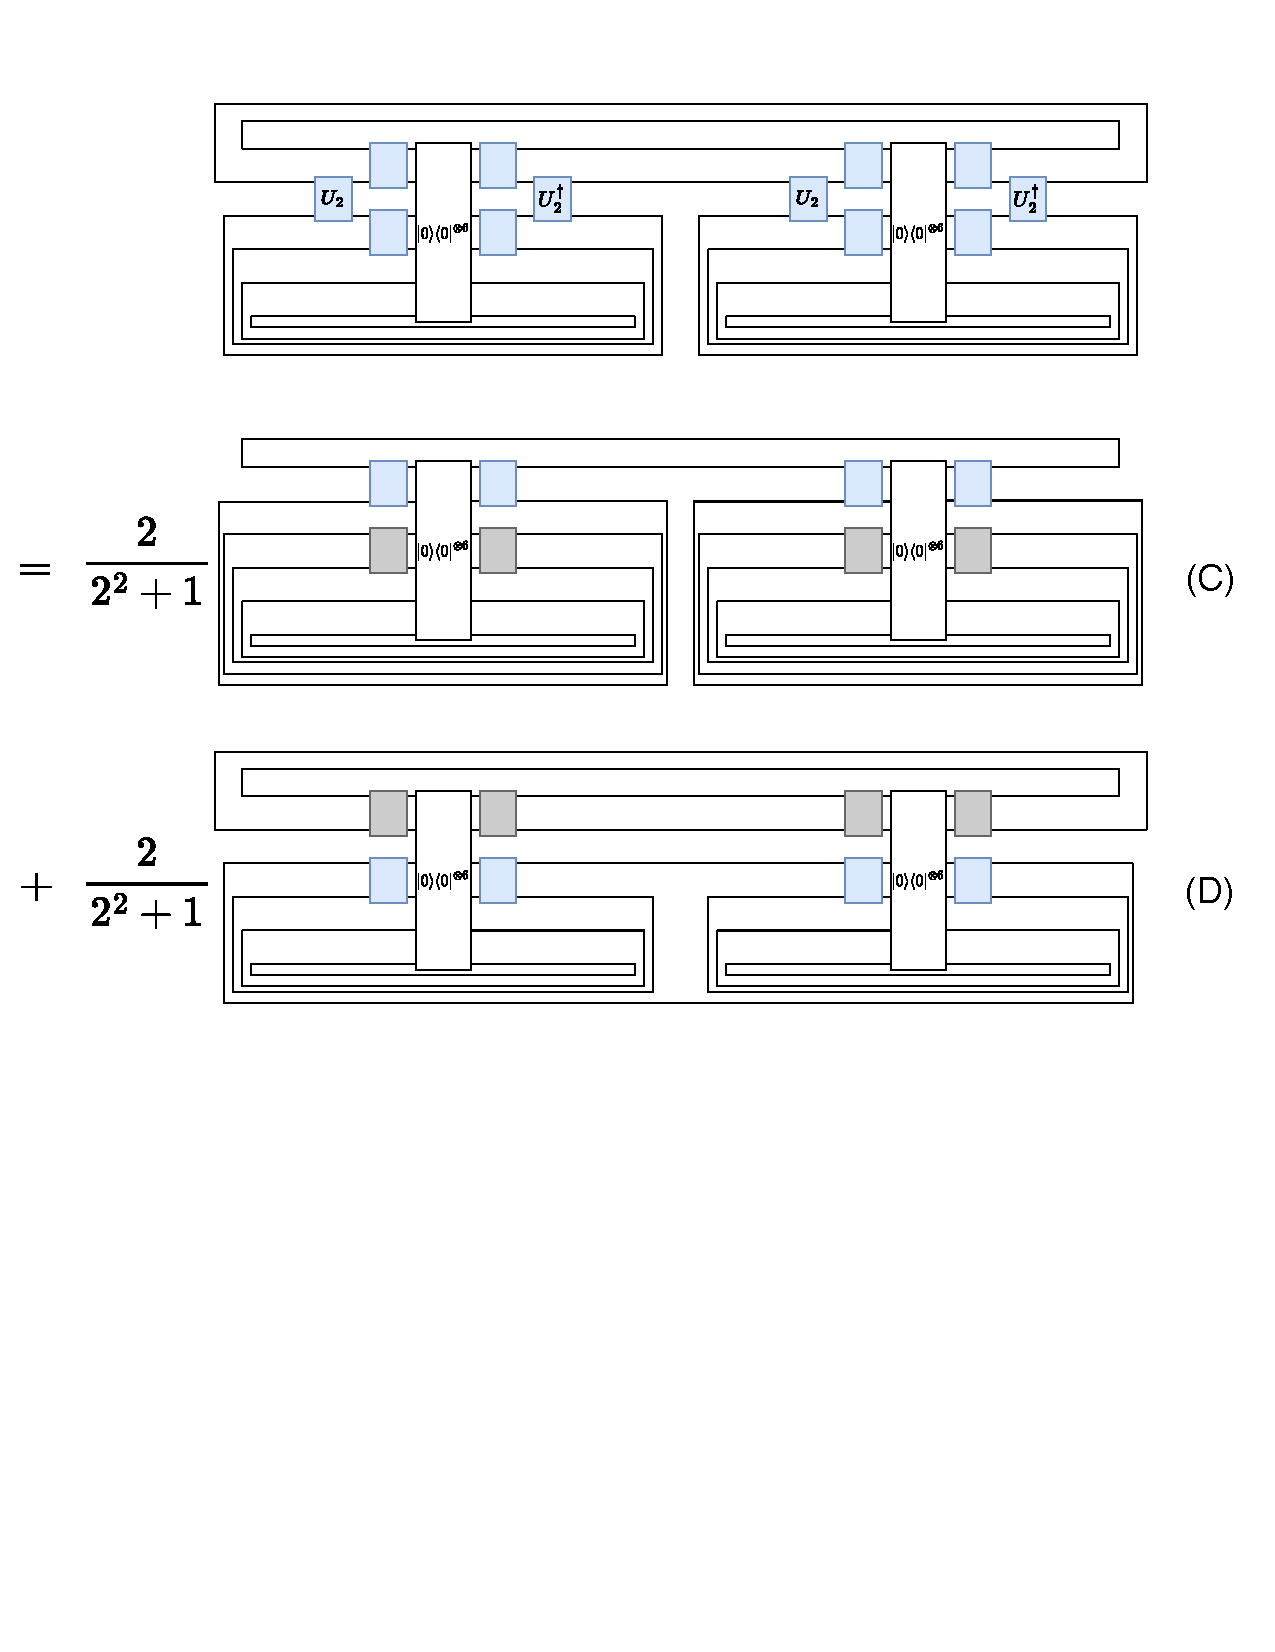
\includegraphics[width=15cm]{int-ALT-Page-2.drawio.pdf}
    \vspace{-20pt}
    \caption{項(B)について、$U_2$ を図~\ref{fig:haar-int-4}を用いて積分した計算の例。}
    \label{fig:tn-alt-int-2}
\end{figure}

以上の計算で出てきた、項(C), (D)は、$UU\dg = \bbid,\,\operatorname{Tr}[\dyad{0}] = 1$ であることを用いると、次の図のようになる。
\begin{figure}[H]
    \centering
    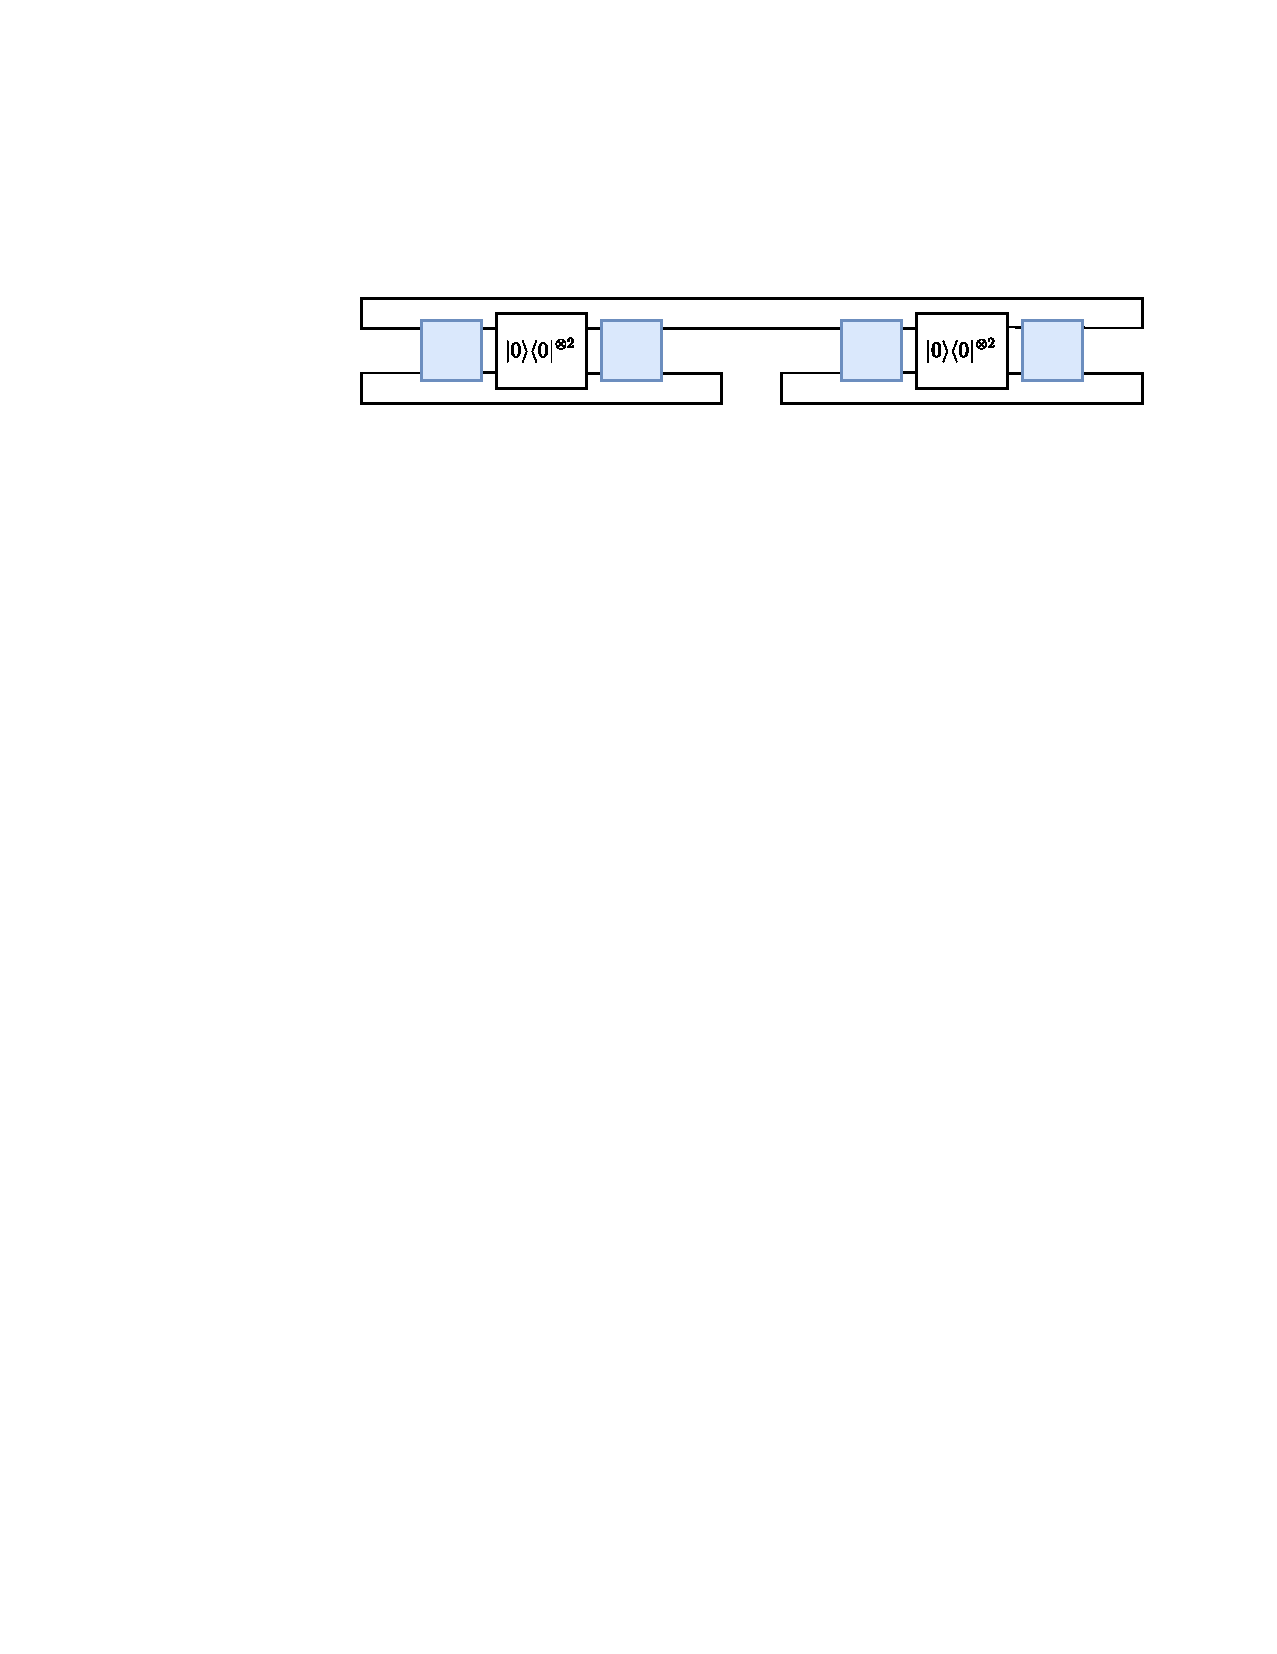
\includegraphics[width=13cm]{int-ALT-Page-3.pdf}
    \label{fig:tn-alt-int-3}
\end{figure}
この計算は、定理\ref{thm:dhs-haar-int}において、$n = 2,\,s = 1$ とした場合に相当するので、$\frac{2^{2-1} + 2^1}{2^2 + 1} = \frac45$ となる。
したがって、$\int_{U\in\bbU} dU \operatorname{Tr}[(\rho^{(h)})^2]$ は、
\begin{align*}
    \int_{U\in\bbU} dU \operatorname{Tr}[(\rho^{(h)})^2]
    &= \frac{2}{2^2 + 1}\times\text{(A)} + \frac{2}{2^2 + 1}\times\text{(B)}\\
    &= \frac{2}{2^2 + 1}\times\text{(A)} + \frac{2}{2^2 + 1}\qty[\frac{2}{2^2 + 1}\times\text{(C)} + \frac{2}{2^2 + 1}\times\text{(D)}]\\
    &= \frac{2}{2^2 + 1}\times1 + \frac{2}{2^2 + 1}\qty[\frac{2}{2^2 + 1}\times\frac45 + \frac{2}{2^2 + 1}\times\frac45]\\
    &= \frac{82}{125}
\end{align*}
\restoregeometry

$\int_{U\in\bbU} dU \operatorname{Tr}[(\rho^{(h)})^2]$ を各層、各量子ビットについて、同様の計算を行った結果が、表~\ref{tab:alt-tr-int} である。これから $\int_{U\in\bbU} dU D_{\HS} (\rho^{(h)} , \bbid/2^{s=1}) = \int_{U\in\bbU} dU \operatorname{Tr}[(\rho^{(h)})^2] - 1/2^{s=1}$ を計算してプロットしたものが図~\ref{fig:hsd-alt-analytical} である。

\begin{table}[H]
    \centering
    \caption{各量子ビット $n$、各層 $L$、$s = 1$ の ALT における $\int_{U\in\bbU} dU \operatorname{Tr}[(\rho^{(h)})^2]$ の計算結果。}
    \label{tab:alt-tr-int}
    \begin{tabular}{c|cccccccc}
        \hline
        $n \backslash L$ & $2$ & $4$ & $6$ & $8$ & $10$ & $12$& $14$ & $16$\\
        \hline
        $2$ & $\frac45$ & $\frac45$ &  $\frac45$ &  $\frac45$ &  $\frac45$ & $\frac45$ & $\frac45$ & $\frac45$ \\
        $4$ & $\frac{18}{5^2}$ & $\frac{394}{5^4}$ & $\frac{9402}{5^6}$ & $\frac{231466}{5^8}$ & $\frac{5757978}{5^{10}}$ & $\frac{143720074}{5^{12}}$ & $\frac{3591166842}{5^{14}}$ & $\frac{89764490986}{5^{16}}$\\
        $6$ &$\frac{18}{5^2}$ & $\frac{386}{5^4}$ & $\frac{8882}{5^6}$ & $\frac{212834}{5^8}$ & $\frac{5210258}{5^{10}}$ & $\frac{128929346}{5^{12}}$ & $\frac{3207308402}{5^{14}}$ & $\frac{79991607074}{5^{16}}$\\
        $8$ & $\frac{18}{5^2}$ & $\frac{386}{5^4}$ & $\frac{8850}{5^6}$ & $\frac{210498}{5^8}$ & $\frac{5116018}{5^{10}}$ & $\frac{125901602}{5^{12}}$ & $\frac{3120244306}{5^{14}}$ & $\frac{77633338882}{5^{16}}$\\
        \hline
    \end{tabular}
\end{table}
